\subsection{Semi-supervised clustering}

\subsubsection{Method}

In Savoy (2014)'s \textit{Estimating the Probability of an Authorship Attribution}~\cite{savoy_probability} they modelized the distribution of the true and false links across the score obtained using a mixture of 2 beta distribution.
Using these two beta distribution models, the position where the area under the curve for both models is maximized (same area under the cut for both models), correspond to the position where the true positive and true negatives are maximized.
Thus, the statistical best possible location whereto separate the rank list if we want to minimize the false positive and false negatives (non-weighted minimization errors).
The idea is to reuse this position for any new rank lists.

To find the position where both beta distribution have the same area under the curve, there might be analytical ways to solve this problematic using the \textit{beta distribution cumulative distribution function analytic form} (beta CDF, probability, area under the curve) but was ignored for this study.
Instead, the equiprobable position is found using a binary search between 0 and 1.
At each step the CDF for the two beta distribution is evaluated until it converges to the same value (or until their difference is a small value, such as $10^{-15}$).
The binary search have a complexity of $O(\log n)$.
With an analytical solve, the complexity could drop to $O(1)$.

As explained in~\cite{savoy_probability} the beta distribution is better suited for authorship problem than the Gaussian distribution since it can grasp a large amount of distribution shapes with its parameters' flexibility.

Since the authors of each document must be known to find the cut.
The idea is here to find the cut location using corpus with known authors and re-use the same value for new corpora.
Thus, turn this method into supervised.

We consider this method as semi-supervised since the only \textit{learnt} parameter is a fixed real number, the distance threshold, and this method do not consider any new corpus for this value computation.
The linkage parameter for this method is the complete linkage, since the cut correspond to the position where the most extremes of the same categories, either true or false links meet.

Figure~\ref{fig:links_score_density} show the distance density for true and false link as well as a beta distribution estimation for St-Jean B rank list generated with text representation 0 (ref. Section~\ref{sec:individual_methods_summary}).
Notice that to be able to modelize the beta distribution, the distances have been normalized between 0 and 1 using Definition~\ref{def:normalization}.

The vertical line indicate the equiprobable position where both beta distribution have the same probability of being a true link and false link (same area under the curve), found using the binary search.
This point can be used as a decision point where the cut should be made in the rank list, this ensures that both false positives and false negatives are minimized.

This technique can be adapted, in the case where the false positives do not have the same importance as false negatives.
The position search criteria can be change such that instead of finding the position where both the true link and false link area correspond to 50\% of their sum (equiprobable case).
It can be generalized such that the true link area represent $\alpha$ and the false link area to $1-\alpha$ with $\alpha \in \left[0,1\right]$.
When $\alpha$ is greater than 0.5, more false positives will occure and less false negatives and when $\alpha$ is smaller than 0.5, more false positives and more false negatives.
The same binary search can be used for this computation, just the target need to be changed.

\begin{figure}
  \caption{Links distances density and beta distribution estimation for St-Jean B with text representation 0}
  \label{fig:links_score_density}
  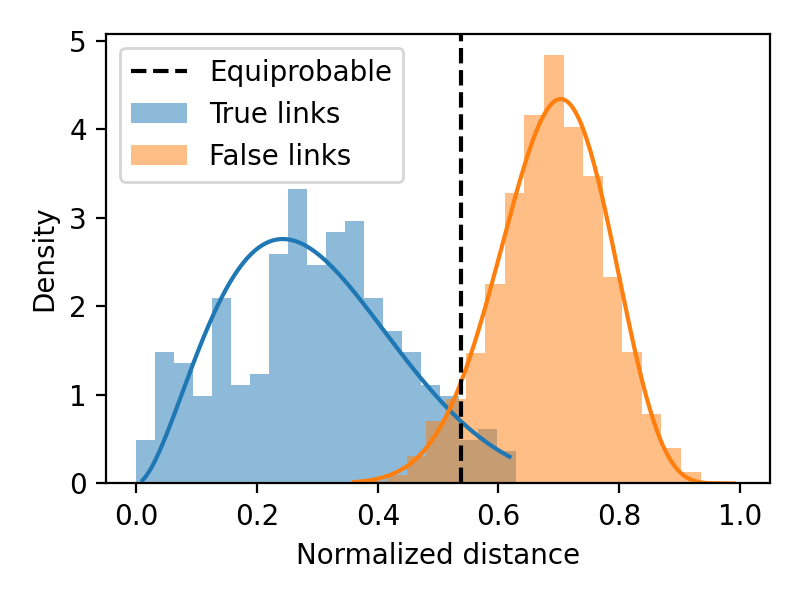
\includegraphics[width=\linewidth]{img/links_score_density.png}
\end{figure}

\subsubsection{Evaluation}

To evaluate the semi-supervised clustering approach, every corpus were used.
First a rank list for each corpus is computed using a Z-Score fusion using the retained rank list, see Section~\ref{sec:annex_retained_text_representation} in annex.
For each rank list, the distance threshold is computed, using the two beta approach, this corresponds to the training phase.
Then for every distance threshold and rank list pair, the clustering is evaluated using the $B^3$ family and the $r_{diff}$.

The distance thresholds found for the Z-Score fusion rank lists for each corpus are in Table~\ref{tab:semi_supervised_clustering_thresholds}
The complete evaluation using Oxquarry, Brunet, St-Jean A and B, is presented in Table~\ref{tab:semi_supervised_clustering_train_test}.
The average values obtained for each metric is presented in Table~\ref{tab:semi_supervised_clustering_average}.

The following conclusions can be drawn with these results:
\begin{itemize}
  \item
  A rather wide range of distance threshold is found depending on the corpus.
  It corresponds to the interval $\left[-0.42, -0.96\right]$ which is 14\% of the interval containing every Z-Scores for these datasets ($\left[-4.79, 2.63\right]$).
  \item
  The average r-ratio is positive, which indicate that this method tends to overestimate the number of clusters, but is really close to find the right number of clusters.
  \item
  The better the average precision of the rank list used is, the better the $B^3_{F_1}$ score seem to be when clustering for this method.
  With an exception for Oxquarry corpus which have better average precision then Brunet (0.84, 0.76) but a lower $B^3_{F_1}$ score in average (0.82 / 0.83) when testing with these corpora.
  \item
  The distance threshold use only have a slight impact when comparing the average $B^3_{F_1}$ score across the corpus.
  The St-Jean A corpus give the best $B^3_{F_1}$ (0.88) and regarding the number of clusters Oxquarry (0.02) seem to be the best corpus for the training.
  This possible difference was already observed in Section~\ref{sec:hierarchical_clustering}, having a slightly greater $r_{diff}$ tends to produce a better $B^3_{F_1}$ score.
\end{itemize}

\begin{table}
  \centering
  \caption{Distance threshold found with the two beta distribution on every corpora when using the Z-Score fusion of the retained rank lists}
  \label{tab:semi_supervised_clustering_thresholds}

  \begin{tabular}{l r}
    \toprule
    Corpus & Threshold \\
    \midrule
    Oxquarry & -0.42 \\
    Brunet & -0.62 \\
    St-Jean A & -0.76 \\
    St-Jean B & -0.96 \\
    \bottomrule
  \end{tabular}
\end{table}

\begin{table*}
  \centering
  \caption{Semi-supervised clustering evaluation}
  \label{tab:semi_supervised_clustering}

  \subcaption{Every possible distance threshold (DT) and retained Z-Score rank list pairs. Metrics in order : $B^{3}_{F_1}$ / $B^{3}_{precision}$ / $B^{3}_{recall}$ / $r_{diff}$}
  \label{tab:semi_supervised_clustering_train_test}
  \begin{tabular}{l l| c c c c}
    \toprule
    \multicolumn{2}{c}{\multirow{2}{*}{}} & \multicolumn{4}{c}{Testing} \\
    \multicolumn{2}{c}{} & Oxquarry & Brunet & St-Jean A & St-Jean B \\
    \midrule
    \parbox[t]{2mm}{\multirow{4}{*}{\rotatebox[origin=c]{90}{DT}}}
    & Oxquarry
    & 0.82/1.00/0.70/0.08
    & 0.81/0.85/0.77/0.07
    & 0.86/0.84/0.87/-0.02
    & 0.91/0.86/0.98/-0.03
    \\
    & Brunet
    & 0.82/1.00/0.70/0.08
    & 0.81/0.85/0.77/0.07
    & 0.87/0.86/0.87/-0.01
    & 0.92/0.88/0.98/-0.02
    \\
    & St-Jean A
    & 0.82/1.00/0.70/0.08
    & 0.85/0.94/0.77/0.09
    & 0.87/0.86/0.87/-0.01
    & 0.97/0.97/0.98/0.00
    \\
    & St-Jean B
    & 0.80/1.00/0.67/0.10
    & 0.84/1.00/0.73/0.14
    & 0.84/0.93/0.77/0.04
    & 0.90/0.97/0.83/0.04
    \\
    \bottomrule
  \end{tabular}

  \vspace{0.5cm}

  \subcaption{Metrics absolute mean}
  \label{tab:semi_supervised_clustering_average}
  \begin{tabular}{l c c c c}
    \toprule
    & $B^{3}_{F_1}$
    & $B^{3}_{precision}$
    & $B^{3}_{recall}$
    & $r_{diff}$ \\
    \midrule
    Testing on Oxquarry               & 0.82 & 1.00 & 0.69 & 0.08 \\
    Testing on Brunet                 & 0.83 & 0.91 & 0.76 & 0.09 \\
    Testing on St-Jean A              & 0.86 & 0.88 & 0.85 & 0.02 \\
    Testing on St-Jean B              & 0.93 & 0.92 & 0.94 & 0.02 \\
    Distance threshold from Oxquarry  & 0.85 & 0.89 & 0.83 & 0.05 \\
    Distance threshold from Brunet    & 0.86 & 0.90 & 0.83 & 0.04 \\
    Distance threshold from St-Jean A & 0.88 & 0.94 & 0.83 & 0.04 \\
    Distance threshold from St-Jean B & 0.85 & 0.98 & 0.75 & 0.08 \\
    \textbf{Global absolute mean} & \textbf{0.86} & \textbf{0.93} & \textbf{0.81} & \textbf{0.05} \\
    \bottomrule
  \end{tabular}
\end{table*}
